
%darc, the Durham Adaptive optics Real-time Controller.
%Copyright (C) 2010 Alastair Basden.

%This program is free software: you can redistribute it and/or modify
%it under the terms of the GNU Affero General Public License as
%published by the Free Software Foundation, either version 3 of the
%License, or (at your option) any later version.

%This program is distributed in the hope that it will be useful,
%but WITHOUT ANY WARRANTY; without even the implied warranty of
%MERCHANTABILITY or FITNESS FOR A PARTICULAR PURPOSE.  See the
%GNU Affero General Public License for more details.

%You should have received a copy of the GNU Affero General Public License
%along with this program.  If not, see <http://www.gnu.org/licenses/>.

\documentclass[a4,10pt]{article}
\providecommand{\gitID}{$Id$}
\usepackage[pdftex,pagebackref=true,colorlinks=true,linkcolor=blue]{hyperref}
\usepackage{xspace}
\usepackage{graphicx}
\newcommand{\ao}{adaptive optics (AO)\renewcommand{\ao}{AO\xspace}\xspace}
\newcommand{\cpu}{central processing unit
  (CPU)\renewcommand{\cpu}{CPU\xspace}\xspace}
\newcommand{\rtcs}{real-time control system (RTCS)\renewcommand{\rtcs}{RTCS\xspace}\xspace}
\usepackage{amsmath}
\newcommand{\ignore}[1]{}
\title{darc: The Durham adaptive optics real-time controller}
\author{Alastair Basden \\ a.g.basden@durham.ac.uk \\ Durham University \\ Department of Physics
  \\ South Road \\ Durham \\ DH1 3LE \\ UK}

\setlength{\textheight}{21.5cm}%
\setlength{\textwidth}{18cm}%
\setlength{\hoffset}{-3.0cm}%
\setlength{\footskip}{1.5cm}%
\setlength{\headsep}{2.5cm}%
\setlength{\voffset}{-2.5cm}%

\begin{document}
\maketitle
{\hspace{7cm} 
\includegraphics[width=3cm]{darclogo.eps}}
\vfill
\gitID
%\section{Quickstart guide}
%%darc, the Durham Adaptive optics Real-time Controller.
%Copyright (C) 2010 Alastair Basden.

%This program is free software: you can redistribute it and/or modify
%it under the terms of the GNU Affero General Public License as
%published by the Free Software Foundation, either version 3 of the
%License, or (at your option) any later version.

%This program is distributed in the hope that it will be useful,
%but WITHOUT ANY WARRANTY; without even the implied warranty of
%MERCHANTABILITY or FITNESS FOR A PARTICULAR PURPOSE.  See the
%GNU Affero General Public License for more details.

%You should have received a copy of the GNU Affero General Public License
%along with this program.  If not, see <http://www.gnu.org/licenses/>.

\begin{verbatim}
QUICKSTART for Paris, Oct 2009

To get the system into a working 2 camera mode:

Plug monitor and keyboard into telemetry server (small HP machine)
Network cable (motherboard) to your external network.
Network cable (PCI) to the local switch.
You will need to configure this machine for external network access.


Boot the telemetry server (small HP machine).
Wait until it has booted (5 minutes to allow crontab time to run).
It logs on automatically.
Open a terminal.
cd /Canary/rtc
./recvStream.py


Plug Network cable on camera PC (black dell machine) into the switch.
Plug the camera fibre into the right hand port.
Plug the camera trigger for the 2 cameras into the cameras and into
the two right hand BNC connectors.
Boot the camera PC (black Dell machine)

Plug network cable on RTC PC (mac pro) into port 1, and into the switch.
Plug the camera fibre into port 0 (right hand port).

Boot the RTC (mac pro).
Log into the RTC as canary twice (ssh from the telemetry server: ssh -X rtc ).
In each, type:
source /Canary/etc/rtc.bashrc
In one type:
cd rtc
./control.py

In the other type:
cd rtc
./startStreams.py -h192.168.0.1

Note - eventually, this should be self-starting, but when we changed
the network config just before shipping it stopped working, so please
do it manually for now.


On the telemetry server, 
open a terminal and type:
cd /Canary/rtc
./rtcgui.py


Make sure that you have a suitable config file (e.g. config2camera.py
or configshakti.py) in /Canary/rtc/ on the telemetry server and in
/home/canary/rtc/ on the rtc machine (mac pro).  

This is currently a bug, which will be fixed (we didn't want to fix it
in the hour before shipping!).

On the GUI, click the start button.  Choose the config file
config2camera.py.  The RTC should then start running.

If working in 1 camera mode, use configshakti.py.

Go to the streams tab, and turn on some streams.  
For example put 100 100 100 in the 3 entry boxes next to rtcPxlBuf.
This sets the decimate rates (for this GUI, out of the RTC between RTC
and tememetry server).
Do this for rtcPxlBuf

Click the spawn plot button.
Select the rtcPxlBuf button in the subscribe too... window, then close
the subscribe too... window.

This will then start showing camera pixels.
To view as an image, type into the text entry box in the bottom left
of the plot:
data.shape=128,256
and then click elsewhere on the screen (so that
the text entry looses focus).
This will show interleaved camera data.
To view from just one camera do either:
data.shape=128,256
data=data[:,::2]
or
data.shape=128,256
data=data[:,1::2]

Any valid python code can be inserted here.  It can be used for
implementing overlays or anything else you wish.

Note, to avoid having to do this, you can set up some plots, and save
them to a configuration file.  Some examples have been done for you -
run the GUI with:
./rtcgui.py initPhaseA.py
A list of available plots then appears in the GUI.
(some of these will work with 2 camera mode, some with 1 camera mode).
These can then be toggled to display or remove plots.

Feel free to edit initPhaseA.py as you wish.

To run some test scripts (some examples of how to do things with the camera):
cd /Canary/local/scripts/test
and look at these scripts.

Note - if any of these scripts require rtc output (pixels/slopes etc),
then the streams need to be turned on in the GUI first, as the script
facility to turn streams on hasn't been implemented yet.


\end{verbatim}


\pagebreak
\tableofcontents
\pagebreak
\section{License}
darc, the Durham Adaptive optics Real-time Controller.
Copyright (C) 2010 Alastair Basden.

This program is free software: you can redistribute it and/or modify
it under the terms of the GNU Affero General Public License as
published by the Free Software Foundation, either version 3 of the
License, or (at your option) any later version.

This program is distributed in the hope that it will be useful,
but WITHOUT ANY WARRANTY; without even the implied warranty of
MERCHANTABILITY or FITNESS FOR A PARTICULAR PURPOSE.  See the
GNU Affero General Public License for more details.

You should have received a copy of the GNU Affero General Public License
along with this program.  If not, see <http://www.gnu.org/licenses/>.

The lead author has a preference that darc should not be used for
military purposes or by organisations with military connections,
however this is not enforceable due to the open nature of the license.

\section{Introduction}
darc, the Durham adaptive optics real-time controller is a generic
controller for adaptive optics systems, and can be configured and
adapted for use with almost any such system.  It has been designed
with low latency as a primary consideration, allowing high performance
\ao to be achieved, with many adjustable parameters being available to
tailor the performance of darc to given hardware and a given \ao
system.

darc was initially designed as a proof of concept to demonstrate that
\cpu based processing on modern processors was sufficient for small
and medium sized \ao systems, negating the need for complex hardware
and long development times.  The success of this demonstration was
such that after some rationalisation and tidying up, darc was made
publicly available.

\subsection{Installation}
Installation of darc follows a standard {\tt make \&\& make install}
process.  The INSTALL file in the release code gives further details
of the dependencies for this process.  Default install location is in
{\tt /opt/darc/}.  

\subsubsection{Interface modules}
darc has a modular architecture, meaning that modularised parts of it
can be swapped in and out and replaced with different modules as
required.  For example, a camera interface module can be produced for
different types of cameras, allowing darc to be suited to a given
hardware setup.  Similarly different mirror interfaces can also be
produced for each deformable mirror required to work with darc.
Wavefront reconstruction, wavefront slope computation and image
calibration are also modularised, allowing darc to be used with any
particular processing algorithms as required by the operator.

To install libraries that are required for your particular
configuration, you must first write them (if they do not exist) using
the templates provided, compile them and install (copy) somewhere pointed to
by your LD\_LIBRARY\_PATH environment variable (/rtc/lib is a standard
location).

\subsection{Running darc}
A single command is required to start darc running: 
{\tt darccontrol PATH/TO/CONFIGFILE}

Note, this requires the omniORB name server (omniNames) to be running in the
location pointed to by your ORBInitRef environment variable, as found
in the darc shell configuration file (rtc.bashrc).

\section{Overview of darc}
The \rtcs contains several main components:
\begin{enumerate}
\item The real-time core (darcmain)
\item A control interface (control.py)
\item Telemetry
\item A graphical engineering interface (darcgui)
\item A scripting interface
\item RTC dynamic libraries (hardware specific)
\item A command line interface
\end{enumerate}

Details of the architecture of darc can be found in Basden et al,
Applied Optics Vol. 49, Iss. 32, pp. 6354–6363 (2010), ``Durham
adaptive optics real-time controller''
Here, a brief description is given.

The real-time core provides a double-buffered parameter buffer in
shared memory, which is accessed by the control interface to control
darc.  The real-time core is written in such a way that no process can
halt or block it, so that jitter can be minimised.  Telemetry data
produced by the real-time core is placed into shared memory circular
buffers, which is then read by clients, with data being sent wherever
necessary.  

The control interface can be accessed by clients using a CORBA
interface, to allow parameters to be changed from anywhere on the darc
accessible network.  An engineering GUI is one such client, which
provides real-time data displays and parameter update facilities.  

Understanding the internals of the real-time core are crucial for
maximising the performance of darc, and so are discussed in further
detail in this document.  

\subsection{The real-time core}

The architecture of the real-time core is descibed briefly here.

The work of processing the data frames is divided between a user
specified number of threads, with each thread assigned work from a
particular camera interface (of course, a given camera interface can
be written to support multiple cameras simultaneously).

The decision to restrict each thread to it's own camera was taken
because the method by which pixels are waited for is not known
(intrinsic to the module itself, which may be third party).  This
may be a blocking call, in which case, if a single thread could serve
multiple cameras, it may be blocked waiting for pixels from one, when
in fact, pixels from all others had arrived.  Time would therefore be
wasted. 

Each thread (one or more per camera) then processes one sub-aperture
at a time (calibration, slope estimation, reconstruction), until all
have been processed, and the wavefront reconstruction has been
completed.  By processing on a sub-aperture basis, latency is reduced,
as the processing of a given frame can start as soon as the pixels for
that sub-aperture have arrived, rather than waiting for the whole
image frame to arrive.  

This is termed a horizontal processing strategy, with all calculation
for a single sub-aperture performed within the same thread, and
reduces latency when compared with a vertical processing strategy, by
reducing the need for thread communication and context switching, and
by improving CPU load balancing.  Fig.~\ref{fig:horiz} demonstrates
this processing strategy, with a vertical processing strategy comparison.

\begin{figure}
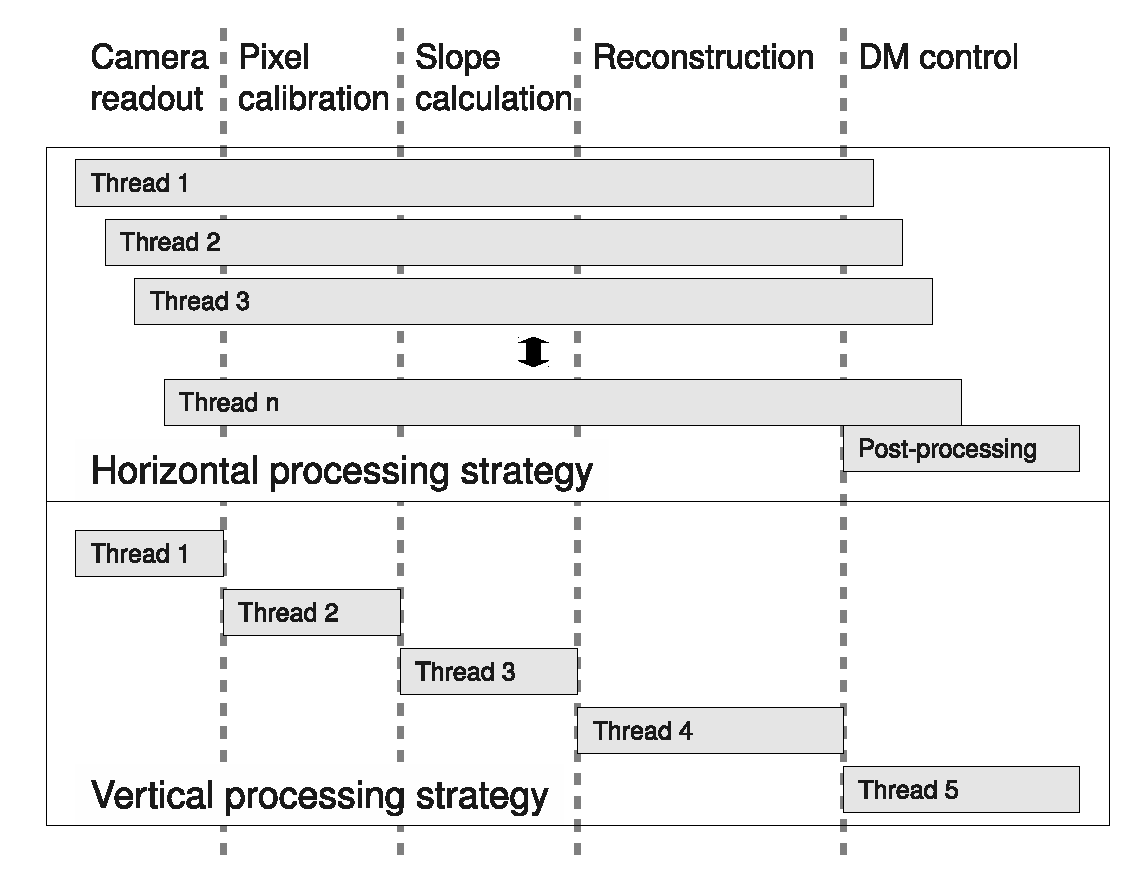
\includegraphics[width=0.5\linewidth]{processingStrategy.eps}
\caption{The thread workload for a horizontal processing strategy (as
  used with darc), and a more conventional vertical processing
  strategy.}
\label{fig:horiz}
\end{figure}

All sub-apertures of a given frame must have been processed before the
next frame is commenced.  Posix mutexes and condition variables are
used as thread synchronisation primatives.  Once the last sub-aperture
has been processed, the wavefront reconstruction is completed and
post-processing then commences (actuator clipping, sending the DM,
etc. as appropriate depending on interface module) while the
sub-aperture processing of the next frame starts (once pixels have
started to arrive).

Best performance is usually achieved by restricting the number of
threads to roughly the number of available processors for larger AO
systems, and less for smaller systems.

\subsubsection{Parameter buffers}
The parameter buffer used to control the RTC is double buffered.  When
a buffer switch is requested, this is carried out by all threads
before the start of a frame, and all new parameters are then swapped
into the real-time core.  The processing time required for a
switch is minimal, and does not significantly increase the
pipeline latency.

Most illegal parameters are caught by the control interface.  However,
due to the modular nature of darc, not all conditions are known, and
so uncaught illegal parameters may have undesired effects, which once
identified should result in safeguards being put in place by the user
to prevent this.

During initialisation, the RTC creates the shared memory parameter
buffers, and then waits for a client to write valid parameters to
them.  The RTC then initialises based on these values, and
commences processing.

\subsection{Modular interfaces}
There are seven modular interfaces to darc, which can be used as
desired:
\begin{enumerate}
\item Camera interface
\item Calibration interface
\item Slope calculation interface
\item Reconstruction interface
\item Mirror interface
\item Asynchronous demand interface
\item Buffer interface
\end{enumerate}


The camera and mirror interfaces are changed depending on hardware
used.  By changing the interface library (on-the-fly), different
cameras and mirrors can be used without having to restart or recompile
the real-time control system.

The calibration interface is used for image calibration, and the
standard library provided can perform background and dark noise
removal, flat fielding and thresholding.

The slope calculation interface computes wavefront slopes from
calibrated images.  The standard library provided performs standard
weighted centre of gravity calculation and correlation calculations
for Shack-Hartmann systems, and can also be used for Pyramid sensor
systems.

The reconstruction interface is responsible for wavefront
reconstruction.  Standard libraries provided with darc are all
matrix-vector based, though alternatives (Fourier and iterative) could
easily be added if required.  A Kalman filter and LQG based reconstruction,
open-loop based reconstruction and conventional closed loop integrator
reconstruction (optionally in GPU) are provided in the darc standard
interface libraries.

A mirror interface library is responsible for taking reconstructed
phase and placing demands on deformable mirrors.  

The asynchronous demand interface makes darc ideal for use as a figure
sensor, receiving asynchronous mirror demands from an open-loop
controller, and performing closed loop control on a non-linear mirror
so that it can be shaped to these demands.

The buffer interface can be used if a user requires the ability to
change parameters on the fly, up to every iteration.  The provided
interface uses a variable in the parameter buffer to achieve this, and
alternative interfaces, for example streaming parameters over a
socket, could also be created.

This modularity is one of the key features of darc, allowing it to be
used in almost any situation, with optional hardware acceleration
where available, and with new or improved algorithms.  Interface
modules can be swapped in the real-time core without halting it,
allowing on-the-fly changes to be made.



\subsection{Parameter changes}
The engineering GUI allows parameters to be set, and allows scripting
to be carried out, e.g.\ interaction matrix generation.

Scripting tools can be written in any language having a CORBA
interface.  The darc project contains a python library which can be
used for scripting, by creating a controlCorba.controlClient() object.

The darctalk command line tool allows getting and setting of
parameters, and reading of telemetry streams.

The darcmagic command line tool implements the darctalk command set
and additional functionality, such as obtaining averaged images and
slopes (averaged in the RTC to guaranteed contiguous), and automated
interaction matrix generation and data logging.  It is also slightly
more intuitive and requires less typing having a more relaxed syntax.

\section{Multiple instances of darc}
It is possible to run multiple instances of darc by setting a unique prefix
name during initialisation.  This name is then pre-pended to shared
memory and the control object.  By specifying -{-}prefix=YOURPREFIX for
the {\tt darccontrol} object and each client, you are able to control
multiple instances of darc.  For example
\begin{itemize}
\item darccontrol configFileTest.py -{-}prefix=test
\item darccontrol configFile.py -{-}prefix=real
\item darcgui -{-}prefix=test
\item darcmagic status -{-}prefix=real
\item etc
\end{itemize}

\subsection{Asynchronous wavefront sensor operation}
The ability to run multiple instances of darc can be used to
facilitate AO systems requiring asynchronous wavefront sensor
operation, i.e.\ wavefront sensors that run at different frame rates
(e.g.\ a fast LGS WFS and a slow tip-tilt WFS).

This is achieved by starting an instance of darc for each wavefront
sensor, using a reconstruction interface that allows partial
reconstruction (for example matrix-vector based reconstruction, such
as libreconmvm.so), and with a mirror interface that can send the
partially computed actuator demands to another instance of darc, for
example over a socket using libmirrorSocket.so, or via shared memory
using libmirrorSHM.so.

Finally, another instance of darc is initialised which is responsible
for collecting together all the partial DM actuator demands, treating
them in the correct way (usually adding them together), and then
sending these final actuator demands to the mirror.  The
libreconAsync.so module performs this task, accepting partial actuator
demands via socket or shared memory, and then adding these to the
current actuator state before sending to the mirror.

If a other protocols are required for this asynchronous
interface, they could easily be developed, for example using sFPDP
communication.  It should be noted that there is no
restriction to where the darc instances are run.  The could be on
separate machines, or all on the same computer (though the communicate
via shared memory, they have to be on the same machine - unless you
have some fancy global shared memory setup).


\subsection{Distributed parallelisation with darc}
In a similar way that darc can be used with asynchronous wavefront
sensors, it can also be distributed across multiple machines by
running an instance of darc on each, responsible for a different
processing stage, with interface modules used to pass appropriate data
between the different darc instances.  For example, you might have one
instance of darc that does pixel calibration.  The slope interface
module could then be used to send calibrated pixels to another
instance of darc that performs the slope calculation, before sending
the slope values to a third instance of darc which performs
reconstruction etc.  In this way, the performance of darc can be
increased.  Note, that in order to do this, some interface module
development may be required by the user.  However, darc provides an
ideal framework in which such parallelisation can be investigated and
tested.


\section{Error handling}
For the purposes of the RTC, we split errors into two types - single
and repeated.  

A single error may for example be a configuration problem.  A repeated
error is one which may keep on arising, for example too many actuators
clipped.  

Errors are written to a circular buffer, which is then read by
clients.  If a repeat error occurs, then a flag is set corresponding
to the error number in the real-time core, and this error will not be
raised again until this flag has been cleared using the clearErrors
parameter.  

Single errors are sent to the clients immediately.  Repeated errors
should only be sent on the first occurrence after a user clear has
occurred.  

For the purposes of errors, the circular buffer is used simply as a
pipe, in which to pipe the errors to {\tt darccontrol} (a real pipe wasn't
appropriate because it may screw up the RTC if it got full).  The
{\tt darccontrol} or telemetry server is then responsible for passing these
errors to clients (upon connection and when new ones occur), and for
deleting/clearing them when requested to do so.  If two clients try to
delete the same error message, then nothing bad occurs, except that if
the error reoccurs between deletions, the second one will also be
deleted, meaning the clients may not see it.  Currently, clients are
not notified if someone else has deleted errors, however this
behaviour would be easy to change if deemed necessary.

\section{Telemetry streams}
Output from the RTC is in the form of telemetry streams.  There are,
for example, a raw pixel stream, a calibrated pixel stream, a slope
measurement stream, an actuator stream, a status stream, etc.
Depending on the interface modules currently in use, other streams may
also be added.  The real-time core places telemetry data into a shared
memory circular buffer which clients can then access and read.

In the case that the available hardware is not powerful enough to
handle all of these streams at full rate, they can be decimated, or
switched off.

There are two points at which decimate values are set.  The first is
the decimate value for the RTC, $d_1$, meaning that the RTC will only
output data every $d_1$ frames (note, this does not affect the AO
loop, only the telemetry frequency).  The other decimate value is that
of the clients, $d_2$, which may be different for each client.  Each value is relative to source, rather than to the
previous decimate value, and the value $d_2$ may be
approximate if it is not a multiple of $d_1$.  For example, if $d_1=5$
and $d_2=8$, then the client will receive every 10 frames rather than
every 8 frames.  However if $d_1$ is then changed to 4, the client
will receive every 8 frames as requested.

Depending on network bandwidth, it is possible to receive every frame
of telemetry data from darc.

To reduce bandwidth requirements, a nodestream.py process can be
started on a remote computer, which simply receives telemetry and
places it into a shared memory circular buffer locally.  Other clients
can then access this buffer, which means that if multiple clients need
one type of telemetry data (for example raw pixel data), the data is
only transferred across the network once, rather than for every
client.  The clients then read the data from the local circular buffers.

The telemetry data produced by darc is readily available in the shared
memory buffers, and so users can easily implement their own standards
for distribution of telemetry, for example using infiniband or a
distributed data service.  The telemetry distribution native to darc
is simple and light weight but may not be ideal for your case.  

\section{Logging and parameter subscription}
Data logging with darc can be performed with the darcmagic command, or
using the Corba interface to initialise a logging connection.
Similarly, parameter subscription is also possible in both of these
ways, to allow a record of the parameter history in darc to be kept,
and to allow a client process to be notified if a given parameter changes.

To perform logging with darcmagic, you would use:

darcmagic read STREAMNAME -n=-1

To keep a record of parameters, you would use:

darcmagic param -file=params.ser

which would write parameters to params.ser in serialised format (use
the serialise library in lib/python to decode this).


\section{Engineering GUI}
The engineering GUI can be used to control the RTC, and to view
telemetry stream data.  It is recommended that a custom GUI should
also be created by darc users to suit the needs of their own system.

Telemetry stream clients (e.g.\ the GUI) have a separate decimate
value from the RTC.  The GUI can
spawn multiple plots, each subscribed to one or more streams as
required.  There is an ability to load and save groups of windows
(including their position and mangle command).  Graphical overlays are
also possible, e.g.\ for sub-aperture masks etc.

The GUI is run with {\tt darcgui [init\_script.py]}

\subsection{GUI Initialisation scripts}
Initialisation scripts can be used when starting the GUI.  These are
Python scripts, which are executed as if they are part of the GUI.  If
one is specified on the command line, this is executed first.  If it
sets ``self.execNext=1'' then the next config file is executed.  This
is ./.rtcguirc.py.  Likewise, if this specifies ``self.execNext=1''
then ~/.rtcguirc.py' is executed, and then (if ``self.execNext=1'' is
set) /etc/rtcguirc.py is executed.  This way, any number between 0-4
files can be executed, depending on whether they exist or not.  More
than one configuration file can be specified on the command line when
starting the GUI.

\subsection{Default plot configuration setup}
When a plot configuration file is specified (load plots button), it
gets added to the plot configuration list.  This is a list of toggle
buttons, which can be clicked to hide or show the associated plots,
making it easy to configure the engineering GUI for a specific AO system.
This list can also be created by a config file, so that there are some
default entries, e.g.\ by putting
self.loadPlotConfig("plotrawpxls.xml") into a config file.

\subsection{Time-series plots}
The standard GUI can be used to plot a time series.
To do this, in the mangle part of a plot, you could put something
like:
\begin{verbatim}
store=makeArr(store,(1000,),"f")
store[:999]=store[1:]
store[999]=data[1]
data=store
\end{verbatim}
This would plot a history of data[1] (assuming len(data.shape)==1)

\subsection{Overlays}
Overlays can be done using the standard GUI.
Simply create an array of shape [x,y,4] called overlay in the mangle,
where the dimensions are for RGBA.  
e.g.
\begin{verbatim}
overlay=numpy.zeros((100,100,4),'f')
overlay[::10,:,::3]=1
overlay[:,::10,::3]=1
\end{verbatim}
would put a red grid on the image.  The shape of the overlay doesn't
need to be the same as that of the image.
In pixel plots, a centroid overlay can also be plotted by toggling the
GUI button.  This only appears when overlay is reshaped, and when
centroids are also being grabbed.

Text and arrows can also be overlain on plots.

\subsubsection{Centroid spots}
Plotting an overlay of centroid spots on pixel images is possible.
For a single camera, the following text can be placed into the mangle
part of the plot window (right click on a plot window to display this,
if it is not visible):
\begin{verbatim}
if streamTime["Cen"][0]!=streamTime["Sub"][0] or \
       streamTime["Cen"][0]!=streamTime["Cal"][0]:
 freeze=1
else:#all frame numbers equal, so plot...
 data=stream["Cal"]
 data.shape=128,128
 import overlayMaker
 if not store.has_key("pattern"):
  store["pattern"]=overlayMaker.makePattern("egg",8)
 pattern=store["pattern"]
 if store.has_key("overlay"):
  overlay=store["overlay"]
 else:
  overlay=None
 overlay=overlayMaker.createSubapCentOverlay(stream,subapLocation, \
                                       pattern=pattern,out=overlay)
 store["overlay"]=overlay
\end{verbatim}

Note, to do this, you must be subscribed to (or have been subscribed
to) rtcCentBuf, rtcSubLocBuf and rtcCalPxlBuf
The shape used for spots can be changed, by setting the pattern
argument.  The oversampling factor can also be changed.

See conf/plotcalimg4cam.xml or similar to have a nice image display.

\subsection{Zernike decomposition}
To plot a zernike decomposition, you can use, in mangle of the mirror
buffer or actuator buffer:
\begin{verbatim}
import zernike
data=zernike.makeZernike(data,10,zernike.Pupil(8,4,0).fn)
\end{verbatim}
This would plot the first 10 zernikes in the case that data
gives the 52 actuators that make up a given mirror, the mask described
by the pupil function.

\subsection{Poke matrix generation}
The GUI or CORBA interface can be used to generate a poke matrix (or
any other response matrix, for example reference slopes).

Creating a response matrix involves putting a set of actuators on the
mirror for a given number of iterations, and averaging the slope
measurements obtained over this time.  This is then repeated for
different actuator sets, and a reponse matrix built up.  Mirror
settling time can be taken account of using this technique.

See the script tag of the GUI for this.

\section{Programs and execution}
There are a number of important processes which are included with
darc.  Here, we detail their usage and command line switches.

\subsection{darccontrol}
{\tt darccontrol} is used to initialise the real-time core, and then
to control it.  {\tt darccontrol} can be stopped and restarted without
affecting the real-time core operation.  If an instance of the
real-time core (with the same prefix) is currently running,
darccontrol will connect to it rather than starting a new instance.

Optional command line arguments include
\begin{center}
\begin{itemize}
\item {\bf -sPREFIX}
\item {\bf -{-}prefix=PREFIX:} Specify a prefix (to create a unique
  identifier for this darc instance).
\item {\bf -aAFFINITY:} Specify the processor affinity for the control
  process.
\item {\bf -iPRIORITY:} Specify the priority (importance) for the control
  process.
\item {\bf -o:} Don't redirect output of darcmain and the control object
  (useful for debugging).
\item {\bf -q:} Used with -o to redirect control output (but not darcmain
  output).
\item {\bf -bBUFSIZE:} Specify the parameter buffer size (default 64MB).
\item {\bf -eHEADERSIZE:} Specify the maximum number of parameters.
\item {\bf -c STREAM NSTORE:} Specify the length of circular buffer for
stream STREAM.
\end{itemize}
\end{center}
You can also specify a configuration filename, config*.py which will
be used if an instance of darcmain is not yet running.

\subsubsection{darcmain}
darcmain is the real-time core part of darc.  It is started
automatically by the control object.  However, if desired, you can
also start it manually instead.  Optional command line arguments include
\begin{itemize}
\item {\bf -bBUFSIZE:} Specify the parameter buffer size (default 64MB).
\item {\bf -sPREFIX:} Specify the prefix.
\item {\bf -i:} Ignore keyboard interrupt.
\item {\bf -r:} Redirect output to /dev/shm/PREFIXstdout.log
\item {\bf -eHEADERSIZE:} Specify the maximum number of parameters.
\end{itemize}

\ignore{
\subsection{darctalk}
darctalk is a process used for querying and altering the state of
darc, as well as receiving telemetry.  It has a strict syntax and was
developed as a command line tool for languages for which no Corba
binding exists, for example Yorick.

darctalk [ init | stop | set | get | read | transfer ] [args] [-{-}debug] [-{-}prefix=PREFIX]

The args specified depend on the initial command.

\subsubsection{init}
-file=configFile.py | -file=configFile.fits

\subsubsection{stop}
No args

\subsubsection{set}
The set command has two formats, either

-telemetry -s=STREAMNAME -d=DECIMATION

to set the decimation rate for stream STREAMNAME to a value of DECIMATION,
or

-name=PARAMNAME [ -file=file.FITS | -string=ASTRING | -value=AVALUE ]
[-comment=COMMENT] [-swap=0/1] [-check=0/1] [-copy=0/1]

where PARAMNAME is the name of the parameter that you wish to change,
with its value specified as a fits file a string or a value.
Optionally, you can add a comment which is tagged with the parameter,
and specify whether you are ready to swap the parameter buffer
(default value 1, set
-swap=0 if you want to delay swapping, for example if you have more
parameters to change).  You can also specify whether you want buffer
checking to be carried out (the default), and whether you wish to copy
the active buffer into the inactive buffer after the swap (default is
1, which should remain, unless you have good reason not to, for
example if you are setting bufferUseSeq parameter).

\subsubsection{get}
The get command has a few formats:
\begin{itemize}
\item {\bf -labels:} Get a list of all parameter names (labels)
\item {\bf -log:} Get the RTC log
\item {\bf -version:} Print version numbers
\item {\bf -telemetry:} Get the decimation rates for all streams
\item {\bf -decimation:} Get the decimation rates for all streams
\item {\bf -name=NAME:} Get the value of parameter NAME
\end{itemize}

What is done with the requested data is then determined by:
\begin{itemize}
\item {\bf -print=1/0:} Print to stdout (default 1)
\item {\bf -file=FILENAME:} Write to file FILENAME in a human readable
  format
\item {\bf -FITS=FITSFILENAME:} Save to a FITS file
\item {\bf -fits=FITSFILENAME:} Save to a FITS file
\end{itemize}

\subsubsection{read}
Read telemetry data from darc.  Arguments are:
\begin{itemize}
\item {\bf -n=N:} Number of iterations (arbitrary maximum limit of 10000 set
  by Zoltan Hubert).
\item {\bf -f=FNO:} Set the starting frame number (specify a negative value
  to wait for this many frames before starting to record).
\item {\bf -d=DECIMATION:} Set the decimation value
\item {\bf -grab:} Grab a single frame
\item {\bf -s=STREAMNAME:} The stream name that you are interested in
\item {\bf -sN=STREAMNAME:} Used if you want to record more than one stream,
  with N being an integer.
\item {\bf -o=OUTPUT:} The output file name.
\item {\bf -oN=OUTPUT:} The output file name corresponding to the Nth stream
  name.
\item {\bf -latest=0/1:} Grab the latest frame.
  from the tail)
\item {\bf -print=0/1:} Print the data
\item {\bf -nosave=0/1:} Set to not save anything.
\item {\bf -myhostname=YOURIP:} Set if you are on a strange platform which
  cannot obtain its own IP address.
\item {\bf -verbose=0/1:} Set verbose mode (prints data)
\item {\bf -binary=0/1:} Print data in binary mode (to allow the output to
  be piped into another process).
\end{itemize}

\subsubsection{transfer}
To transfer a file from the local PC to darc, you can use

darctalk transfer -file=LOCALFILENAME [-remote=REMOTEFILENAME]

where the remote filename defaults to the local filename if not
specified.  Why do we have this command?  It was implemented to give a
simple way of transferring files by script, without needing to setup
NFS or passwordless ssh.
}


\subsection{darcmagic}
{\tt darcmagic} is a process used for querying and altering the state of
darc, as well as receiving telemetry.  It has a loose syntax aimed at
being more convenient for command line usage.

darcmagic [ set | get | read | init | convert | labels | decimate |
  average | grab | poke | stop | print | transfer | release | status |
  swap | param | log | error | splitter | summer | time ] [args] [-{-}debug] [-{-}prefix=PREFIX]

The args specified depend on the initial command.

\subsubsection{set}
darcmagic set [-name=NAME | NAME] [-file=FILE |
  -string=STRING | -value=VALUE | VALUE ] [-comment=COMMENT]
[-swap=1/0] [-check=1/0] [-copy=1/0] 

where NAME is the name of the parameter that you wish to change or set,
with its value specified as a fits file, a string or a value.
Optionally, you can add a comment which is tagged with the parameter.
The swap parameter specifies whether you are ready to swap the parameter buffer
(default value 1, set
-swap=0 if you want to delay swapping, for example if you have more
parameters to change).  You can also specify whether you want buffer
checking to be carried out (the default), and whether you wish to copy
the active buffer into the inactive buffer after the swap (default is
1, which should remain, unless you have good reason not to, for
example if you are setting bufferUseSeq parameter).

Note, the simpler usage: darcmagic set NAME VALUE is possible.

\subsubsection{get}
darcmagic get [-labels | -log | -version | -decimation | -name=NAME |
  NAME] [-comment=0/1] [-cmd=CMD] [-print=1/0] [-file=FILE]
[-FITS=FITSFILE] [-plot=0/1]


The get command has a few formats:
\begin{itemize}
\item {\bf -labels:} Get a list of all parameter names currently in darc (labels)
\item {\bf -log:} Get the RTC log
\item {\bf -version:} Print version numbers
\item {\bf -decimation:} Get the decimation rates for all streams
\item {\bf -name=NAME:} Get the value of parameter NAME
\end{itemize}


The -cmd
option allows the user to specify python syntax for operating on the
data prior to saving or printing.  The -plot=1 option displays a plot
of the data.

{\tt darcmagic get rmx -cmd=''print value.shape; value=value[:10]'' -plot}

would print the shape of rmx, then select the first 10 elements and
plot them.

\subsubsection{read}
Obtain telemetry data from darc.

darcmagic read [-n=N] [-f=FRAMENO] [-d=DECIMATE] [-grab=0/1] [-{-}save-on-fly]
[-local=0/1] [-binary=0/1] [-myhostname=HOSTNAME] [-s=STREAM |
  -sN=STREAM | STREAM] [-o=STREAM.FITS | -oN=STREAM.FITS |
  STREAM.FITS] [-latest=0/1] [-print=0/1] [-nosave=0/1] [-verbose=0/1]
[-asfits=0/1] [-sendFromHead=0/1] [-plot=0/1] [-cmd=CMD]

Arguments are:
\begin{itemize}
\item {\bf -n=N:} Number of iterations.
\item {\bf -f=FNO:} Set the starting frame number (specify a negative value
  to wait for this many frames before starting to record).
\item {\bf -d=DECIMATION:} Set the decimation value
\item {\bf -grab:} Grab a single frame via the control, rather than
  telemetry, interface.
\item {\bf -s=STREAMNAME:} The stream name that you are interested in.
\item {\bf -sN=STREAMNAME:} Used if you want to record more than one stream,
  with N being an integer.
\item {\bf -o=OUTPUT:} The output file name.
\item {\bf -oN=OUTPUT:} The output file name corresponding to the Nth stream
  name.
\item {\bf -latest=0/1:} Grab the latest frame (from the tail)
\item {\bf -print=0/1:} Print the data
\item {\bf -nosave=0/1:} Set to not save anything.
\item {\bf -myhostname=YOURIP:} Set if you are on a strange platform which
  cannot obtain its own IP address.
\item {\bf -verbose=0/1:} Set verbose mode (prints data)
\item {\bf -binary=0/1:} Print data in binary mode (to allow the output to
  be piped into another process).
\end{itemize}


The -cmd option is as with the ``get'' command, the save-on-fly option
allows data to be streamed to disk rather than gathered in memory, and
there is no arbitrary limit to the number of frames that can be
received.  If N is -1 (-n=-1) then recording will go on indefinitely
until stopped.  In the case that more than 10000 frames are requested,
data will be streamed to disk.  By default, streaming to disk is in a
darc specific format, however, if -asfits=1 is specified, it is
streamed to disk as FITS format with slightly greater CPU consumption.
Note, when the recording finishes, it will be converted into FITS
format automatically unless interrupted.

If -local=0 then data is obtained via a new socket, rather than from
local circular buffers.

If sendFromHead=1 then the head of the circular buffer is read,
meaning that frames might be lost, however the data is always the most
recent.  This should be selected for live image displays.

\subsubsection{init}
Initialise darc.

darcmagic init [-file=FILE | FILE] [-remote=0/1]

If remote is specified, the file is treated as being available on the
RTC machine, not on the local machine.

\subsubsection{convert}
Probably unnecessary, but can be used to convert a darc specific
format telemetry stream data into FITS format.

darcmagic convert FILE.log


\subsubsection{labels}
darcmagic labels -print=1/0

Prints the available parameter names.

\subsubsection{decimate}
darcmagic decimate [-s=STREAM | STREAM] [-d=DECIMATION | DECIMATION]

Set the decimation rate to DECIMATION for stream STREAM.

\subsubsection{average}
darcmagic average [-s=STREAM | STREAM] [-n=N | N] [-w=0/1]
[-print=0/1] [-file=FILE.fits] [-plot=0/1]

where STREAM is rtcCalPxlBuf or rtcCentBuf, will result in taking the
average of N iterations of data.  If w=1 it will be the whole
calibrated image (don't do this if the loop is closed), otherwise will
be just parts of the image that are used by data processing.

\subsubsection{grab}
Grabs a single frame of telemetry data.

darcmagic grab [-s=STREAM | STREAM] [-latest=0/1] [-cmd=CMD]
[-print=0/1] [-tostring]

If -tostring is given, converts this data to a string and prints it.

darcmagic grab rtcStatusBuf -tostring

\subsubsection{poke}
A rudimentary interaction matrix generation routine.

darcmagic poke [-v=V -ignore=IGNORE -hold=HOLD -acts=ACTS.fits] |
[-steps=STEPS.fits]  -rcond=RCOND] [-print=0/1 -file=FILE.fits -plot=0/1]

Creates an interaction matrix with perturbation size V, ignoring
IGNORE frames after setting an actuator and then integrating for HOLD
frames.  If ACTS.fits is specified, this file contains the poking
pattern, otherwise it will be generated using V, IGNORE and HOLD.  If
ACTS.fits is specified and STEPS.fits is specified then STEPS.fits
contains the number of iterations to hold at each stage.

If RCOND is specified, this is treated as a floating point
conditioning value, and the control matrix is then generated.
FILE.fits is the output filename which if RCOND is specified is a
multi-HDU file.

If plot=1, the interaction matrix is plotted.

\subsubsection{stop}
Stop darc real-time core.

If {\tt darcmagic stop -c} is specified, this will also stop the
control interface, which must then be restarted by a new call to {\tt
  darccontrol}.

\subsubsection{print}
Provides a printout of the current parameters in darc.

darcmagic print [-print=1/0] [-file=FILE]



\subsubsection{transfer}
{\tt darcmagic transfer -file=LOCALFILENAME [-remote=REMOTEFILENAME]}

where the remote filename defaults to the local filename if not
specified.  Why do we have this command?  It was implemented to give a
simple way of transferring files by script, without needing to setup
NFS or passwordless ssh.


\subsubsection{release}
Release the control lock (useful if something has gone wrong)

\subsubsection{remove}
darcmagic remove [-name=NAME | NAME] [-return=1/0] [-doSwitch=1/0]
[-print=1/0] [-file=FILE] [-FITS=FILE.fits]

Remove a parameter from the buffer, optionally returning it (and then
printing and saving it as requested).  If doSwitch is set, the buffers
are swapped.

\subsubsection{status}
Print out the current status of darc
\subsubsection{swap}
darcmagic swap NAME1 NAME2 [-swap=1/0]

Swap the values in NAME1 and NAME2, and then (if swap!=0) do a buffer
swap to update the RTC.

\subsubsection{param}
darcmagic param [-file=FILE] [-print=1/0]

Subscribe to changes in the parameter buffer, then printing or saving
details whenever a change occurs.  This allows logging of the
parameter buffer to occur.

\subsubsection{log}
Read the darc logs.  Ctrl-C must be used to exit.

\subsubsection{error}
Print or remove any errors within darc.  Args can be [clear [error string |
    -e=error string]] [-print=1/0] [-file=filename.txt [-log=0/1]

\subsubsection{splitter}
Creates a new telemetry stream that is a subset of an existing one.

Args can be [start stream from to [step [block size]]] | [stop name] |
[list]

Here, step is the row skip, and block is the block size.  e.g.
{\tt darcmagic splitter start rtcPxlBuf 10 200 2}

The name (used in {\tt darcmagic splitter stop}) is obtained when
starting a split stream, or from {\tt darcmagic splitter list}.

\subsubsection{summer}
Creates a new telemetry stream that is the sum of a history of an
existing steram.  This new stream will contain the last {\tt nsum}
frames of the original summed together.


Args can be [start stream nsum [rolling? [dtype [nstore [set parent decimate (default 1) [start variance stream (default 0, actually a data**2 stream)]]]]]] | [stop name] | [list]

\subsubsection{time}

Measure the current frame rate.  Args can be [nframes] [-s] where -s
specifies that standard deviation should also be computed.  If nframes
is <0 will continuall compute and report.  If -s not specified and
nframes>0, only the final mean is returned, not the time of every
frame, reducing network bandwidth usage.



\subsection{darcgui}

The engineering GUI, with the following parameter options:
\begin{itemize}
\item {\bf -b BUFSIZE:}
\item {\bf -{-}bufsize=BUFSIZE:} Specify the buffer size to be
  used locally
\item {\bf -c configfile.py:}
\item {\bf -{-}config=configfile.py:} Specify the
  configuration file used to configure the GUI.
\item {\bf -h:}
\item {\bf -{-}help:} Print a help message
\item {\bf -n:} Don't request comments when sending newly changed
  parameters.
\item {\bf -s PREFIX:}
\item {\bf -{-}prefix=PREFIX:} The prefix for the RTC that you
  wish to connect to.
\end{itemize}

\subsection{splitter}
Splits a telemetry stream into a new smaller one.  All local, writing
to shared memory.  Usually started using darcmagic/API.

\subsection{sender}
Sends a telemetry stream from a shared memory circular buffer over the
network to a receiver using TCP/IP point-to-point connection socket.
Usually started using darcmagic/API.
\subsection{receiver}
Receives a telemetry stream over a socket and writes it to a shared
memory circular buffer.  Usually started using darcmagic/API.

\subsection{summer}
Sums a telemetry stream for a given number of frames (optionally
rolling), and writes the result to a new telemetry stream.  Can
optionally also sum the square of the data (producing another
telemetry stream), which is useful for obtaining the variance of the data.
Usually started using darcmagic/API.

\ignore{
\subsection{nodestream.py}
A process which receives telemetry data for one particular stream from
darc and writes it to a local shared memory circular buffer.  This
buffer can then be accessed by lots of clients without consuming more
network bandwidth.

nodestream.py NAME [PREFIX]
}



\section{The parameter update interface}
darc has the ability to update any parameter on a frame by frame
basis, using a buffer shared library.  This library is dynamically
loaded into the RTC, and of course can be unloaded and changed by the
user to suit their requirements.  The standard buffer update library,
librtcbuffer.so, uses an entry in the parameter buffer called
``bufferSeq'', and interprets this as a sequence of data to be used by
the RTC.  The user could write an alternative version that accepts new
parameters via a socket or shared memory etc, and then load this into
the RTC.

The contents of the bufferSeq array are a series of headers and data
units.  The headers are composed of four 32 bit integers, with values
being: Header size (32), Number of entries in the data, Number of
iterations before moving onto the next set in the series, and the size
of the header plus the data (so the pointer to the next set in the
series).

Each data section is organised as a parameter buffer and interpreted
as such, with one caveat:  If the length of the comment for a
particular variable is zero, this means change the active parameter
contents, while if non-zero, this means change the inactive parameter
buffer contents.

Arrays can generally be written to the active buffer (so long as they
aren't used by the pre or post processing threads), while other values
should be placed into the inactive buffer, and then
``switchRequested'' set in the active buffer, so that the RTC does a
buffer swap and switches them into action.  Once the end of the series
of buffers is reached, the RTC wraps around back the the beginning (if
this isn't the desired behaviour, then ``bufferUseSeq'' can be unset
in the inactive buffer as the last step in the sequence).  

If you wish to change parameters on a frame by frame basis, and these
aren't arrays (so, you must initiate buffer swaps each time), then
when setting ``bufferUseSeq'' to one, to start the sequence, you
should make sure that the copy flag is set to zero, so that active
buffer contents are not copied into the inactive buffer (which by that
time may be active).  This is achieved for example using
{\rm darctalk set -name=bufferUseSeq -value=1 -copy=0}  or, using the
{\rm ctrl=darc.control()} object by using {\rm
  ctrl.set(``bufferUseSeq'',1,copy=0)}.  In this case, you should also
ensure that during the first iteration, the bufferUseSeq in the
inactive buffer is also set to 1.

You should take care not to do other RTC operations that will involve
a buffer copy or swap while the sequence is running.

Note, if you wish to have a sequence of actuators, this can be done
simply by specifying a larger ``actuators'' array.  This is a special
case, and the buffer update interface is not required.

To create a suitable ``bufferSeq'' array using python, the following
code will work (and will alternate the reference slopes used by the RTC).

\begin{verbatim}
import buffer
import darc

bs=buffer.BufferSequence()
bs.add("refCentroids",numpy.ones((288,),"f"),0)
bs.add("refCentroids",numpy.ones((288,),"f")*0.5,1)
bufseq=bs.makeBuffer(2)

ctrl=darc.control()
ctrl.set("bufferSeq",bufseq)
ctrl.set("bufferUseSeq",1,copy=0)
\end{verbatim}

To create a suitable ``bufferSeq'' array for a non-array parameter,
you could use:
\begin{verbatim}
import buffer
import darc

bs=buffer.BufferSequence()
bs.add("useBrightest",5,0,inactive=1)
bs.add("useBrightest",25,1,inactive=1)
bs.add("useBrightest",0,2,inactive=1)
bs.add("switchRequested",1,0)
bs.add("switchRequested",1,1)
bs.add("switchRequested",1,2)
bufseq=bs.makeBuffer(3)

ctrl=darc.control()
ctrl.set("bufferSeq",bufseq)
ctrl.set("bufferUseSeq",1,copy=0)
\end{verbatim}

Awesome!




\section{RTC configuration}
The real-time control system is configured during initialisation using
a configuration file, and parameters can then be changed at
any time during operation by writing to a parameter buffer in shared
memory.  A client will do this via the control process.

The list of parameters that can be used to configure darc is described
here.  Note that some of these are specific to particular interface
modules, and so not all are always required.  To create a new
configuration file it is generally easiest to start with an existing
one, which are located in {\tt /opt/darc/conf} (or wherever darc has
been installed).


\subsection{ncam}
This is the number of camera objects in the system (note, not
the number of cameras necessarily, as multiple cameras can be combined
into one camera object).  For example for CANARY phase 0, this will be
1, while for CANARY phase A, this will be 2 (3 WFS, 1 truth sensor,
combined into 2 pixel streams).  This should not be changed for the
duration of the real-time control system.

Type int32

\subsection{nacts}
The total number of actuators for the system.  

Type int32

\subsection{nsub}
An array with ncam entries, specifying the number of sub-apertures for
each frame grabber.

Type array,int32,shape=ncam

\subsection{npxlx}
An array of length ncam, specifying the number of pixels in a
horizontal direction with an entry for each frame grabber.

Type array,int32,shape=ncam

\subsection{npxly}
An array of length ncam, specifying the number of pixels in a
vertical direction with an entry for each frame grabber.

Type array,int32,shape=ncam



\subsection{subapLocType}
Defines the type of subapLocation used.


\subsection{subapLocation}

An important structure, specifying the layout of sub-apertures for the
system.  

If subapLocType is zero, then subapLocation is an array of shape (nsubaps,6) where nsubaps is the
total number of sub-apertures (valid and invalid) for the system.
This can be computed by (nsubx * nsuby).sum().  For each sub-aperture
there are then 6 values,
$[y_{start},y_{end},y_{step},x_{start},x_{end},x_{step}]$.  These are
the pixel values that the sub-aperture starts and finishes at, and the
number of rows or columns to step.  With interleaved pixel data from 2
cameras, $x_{step}$ should be 2.  

Type array,int32,shape=totSubaps,6

If subapLocType is one, then subapLocation is an array of shape
(nsubaps,N), where N is the maximum number of pixels per subaperture.
The entries in this array are then the pixel numbers of pixels in this
sub-aperture, or -1 for entries where the number of pixels is less
than N.  This can be used to create arbitrary shaped sub-apertures.
Although present in darcmain, this is not well supported by interface
modules, so care should be taken if subapLocType is to be set to one.

Type array,int32,shape=totSubaps,N

\subsection{windowMode}
Should be a string either ``basic'', ``adaptive'' or ``global'' to
switch between basic, adaptive or global windowing mode (affecting
whether sub-apertures follow spots).

Type string

\subsection{subapFlag}
An array of size equal to the total number of sub-apertures, with a
flag value for each, specifying whether this sub-aperture should be
used.

Type array,int32,shape=totSubaps

\subsection{go}
When set to zero, the RTC will stop and exit.

Type int32

\subsection{pxlCnt}
An array of size equal to the total number of sub-apertures.  The
entries are the total number of pixels that are required for each
sub-aperture before processing of this sub-aperture can commence.
Note this can be computed from subapLocation though is given as a
parameter to allow extra flexibility.  To allow the RTC to process
multiple sub-apertures before commencing reconstruction, these
sub-apertures should have the same pxlCnt value.

Type array,int32,shape=totSubaps

\subsection{pause}
A flag, which if set pauses the RTC (though camera frames are still
read).  No image calibration, slope calculation or DM vector
computation is carried out.

Type int32

\subsection{printTime}
Primarily for debugging, if set, the RTC will print the frame time.

Type int32

\subsection{ncamThreads}
An array of length ncam, with a value for each frame grabber
specifying the number of threads for each.  Use this to fine tune RTC
performance.  Should not be altered after initialisation.

Type array,int32,shape=ncam

\subsection{switchRequested}
When set, the RTC will switch parameter buffers.

Type int32

\subsection{actuators}
A user defined array of actuators, of size equal to the number of
actuators times some value.  These will be placed on the mirror as
sets of actuators in turn, either replacing RTC
computed values, or added to them (possibly with a mask).

Type None

Type array,float32,shape=N,nacts where N is the number of entries in
your sequence (can be 1)


\subsection{threadAffinity}
An array of length equal to 1 + ncamThreads.sum().  A value for each
thread (the first being the post-processing thread) defining a CPU
mask for where the threads should be allowed to run.  Use this to fine
tune the RTC.

Type None

Type array,int32,nthreads+1

\subsection{threadPriority}
An array of length equal to 1 + ncamThreads.sum().  A value for each
thread (the first being the post-processing thread) defining the
thread priority.  Use this to fine tune the RTC.  It the RTC is not
run with the correct permissions, this will be ignored (will print
out a warning message).  Typically, the RTC should be run as root to
allow this to be used.

Type None

Type array,int32,nthreads+1



\subsection{delay}
An optional delay in microseconds, for debugging purposes to slow the
RTC down when no real cameras are attached.

\subsection{clearErrors}
Used by the error handler in the GUI to acknowledge errors.

\subsection{camerasOpen}
A flag used to open the camera shared object library
(e.g. librtccamera.so).  

\subsection{cameraParams}
An array of 32 bit integers which is passed into the camera object to
configure it.  The values in this array depend on which camera library
is used.  For example, if using the FITS file reader camera object
libcamfile.so, this is just the filename
(e.g. numpy.fromstring(``shimage.fits'',dtype=numpy.int32)), while for
the SL240 interface, this has 5 x ncam values and a few more optional
values for configuration.  The per-camera values are equal to
[blocksize, timeout, port, affinity, priority] for each camera, where
blocksize is the number of pixels that should be read as a block
(usually a few rows at a time).  Timeout is the time to wait if data
is not received before raising an error and trying again.  Port is the
SL240 fibre port, numbered from 0 being closest to the motherboard for
Curtiss Wright cards.  Affinity is the thread CPU affinity and
priority is the thread priority for this frame grabber.

\subsection{cameraName}
The name of the camera object expected from the shared object library.
This will raise an error if not actually in the camera library.

\subsection{mirrorOpen}
A flag specifying whether the mirror library is in use or not.

\subsection{mirrorName}
The name of the mirror object expected from the shared object library.
This will raise an error if not actually in the mirror library.

\subsection{frameno}
Updated by the RTC, the frame number at which a buffer switch last
occurred.

\subsection{frameTime}
Updated by the RTC, the time at which a buffer switch last occurred.

\subsection{nsteps}
If greater than zero, the number of iterations to run the RTC for
before pausing.  Used in debugging.  Set to -1 to run indefinitely.

\subsection{closeLoop}
A flag, whether the loop should be closed (values sent to DM) or not.

\subsection{mirrorParams}
The parameters supplied to the mirror library, an array of 32 bit
integers, contents depending on the mirror library.  For the SL240
mirror library, there are 4 values, being the timeout, port, thread
CPU affinity and thread priority.

\subsection{addActuators}
Whether user defined actuators should replace (if 0) RTC computed
values, or add (if 1) to them.

\subsection{actSequence}
When actuators are specified, actSequence defines the number of times
each set of actuators should be placed on the mirror.  This size of
this array should be equal to the number of sets of actuators
specified.

\subsection{recordCents}
Used to compute an interaction matrix or reference slopes.  If set,
slope measurements are recorded and avereged while an actuator
sequence is played.


\subsection{averageImg}
Used by GUI/in scripting, The number of frames to average calibrated
images for before publishing the result to the generic stream.

\subsection{slopeOpen}
A flag determining whether the slope
shared object library is in use.

\subsection{slopeParams}
c.f.\ cameraParams

\subsection{slopeName}
c.f.\ cameraName

\subsection{actuatorMask}
A mask of size equal to the number of actuators to specify which user
defined actuators should be used.

\subsection{dmDescription}
Currently used only by the GUI, for DM control.

\subsection{averageCent}
As with averageImg, equal to the number of frames to average centroids
too before publishing the result once to the generic stream.


\subsection{comment}
An optional comment added to the buffer.  It would be hoped that
a sensible comment can be added when the user updates the buffer.
e.g.\ to specify the change they made.  It should also be noted that
each parameter in the buffer can also have an attached comment.



\subsection{figureOpen}
Whether the figure sensor library is open or not (user and RTC
settable).

\subsection{figureName}
The name of the figure sensor library, if using RTC in a figure
sensing mode.

\subsection{figureParams}
Parameters to be passed to the figure sensor library at open time.

\subsection{reconName}
Name of the reconstructor library.



\subsection{reconlibOpen}
Whether the reconstructor library is open (set to 1 to open it, and if
it is still 1 once the RTC has tried to open it, you know that the
open was successful).

\subsection{bufferOpen}
Whether the buffer interface library is open.

\subsection{bufferName}
Name of the buffer interface library to use, e.g.\ librtcbuffer.so

\subsection{bufferUseSeq}
Whether buffer sequencing should be active.

\subsection{subapAllocation}
None, or an array specifying a thread number for each sub-aperture,
the thread number that is to be used to process this sub-aperture.
Used for optimising performance and reducing latency.  If not set,
then threads are assigned a sub-aperture to process when they have
finished previous processing.

\subsection{noPrePostThread}
0 or 1 a flag used to determine whether a separate pre and post
processing thread should be used, or whether these operations should
be carried out by a sub-aperture processing thread.  This defaults to
zero, but can be used for optimising performance.

\subsection{iterSource}
Specifies the source for the iteration number to be used by darc.
A 32 bit integer with the lowest 16 bits corresponding to the source
(0 internal source, 1 camera interface, 2 calibration interface, 3
slope interface, 4 reconstructor interface, 5 mirror interface, 6
figure sensor interface, 7 buffer interface) and the upper 16 bits
corresponding to the index of the source.  Note, the interface
libraries are able to generate an arbitrary number of frame numbers
each, and the index is used to select one of these.  The selected
iteration number is then used for darc telemetry. 


\subsection{Calibration interface (librtccalibrate.so)}
The following parameters are used by the standard calibration module.  
\subsubsection{powerFactor}
A value to raise pixel values to the power of.  Used only by the
calibration interface module.  

Type float

\subsubsection{bgImage}
The background image (or None).  Size should be equal to the total
number of pixels from all cameras, and pixel ordering should be as
received by the RTC.  Used only by the calibration interface module.

Type None

Type array,float32,shape=npxls

\subsubsection{darkNoise}
The dark map image (or None).  Used only by the calibration interface module.

Type None

Type array,float32,shape=npxls

\subsubsection{flatField}
The flat field image (or None).  Used only by the calibration interface module.

Type None

Type array,float32,shape=npxls

\subsubsection{thresholdAlgo}
The thresholding algorithm to be used.  If equal to 1, 
values less than the threshold are set to zero.  If equal to 2, the
threshold is subtracted from all values, and negative values are set
to zero.  Other values mean no thresholding.  Used only by the calibration interface module.

Type int32

\subsubsection{thresholdValue}
The value use for thresholding.  This can be either a single value, or
an array of size equal to the total number of sub-apertures, with a
value per sub-aperture.  Used only by the calibration interface
module.

Type float

Type array,float32,shape=totSubaps

\subsubsection{pxlWeight}
The pixel weighting factor, an array of values to multiply pixels by.
This allows weighted centre of gravity algorithms to be used.

Image calibration is performed using
\begin{enumerate}
\item Dark noise subtraction
\item Flat field multiplication
\item Background subtraction
\item Application of threshold
\item Multiplication by pixel weighing
\item Application of power factor.
\end{enumerate}

\subsubsection{fakeCCDImage}
For testing, if specified, a fake CCD image.

Type None

Type array,int32,shape=npxls

\subsubsection{calmult}
Used internally
\subsubsection{calsub}
Used internally
\subsubsection{calthr}
Used internally

\subsubsection{imgGain}
A gain factor (default of 1, can be between 0 to 1, or an array of
values, one for each sub-aperture) that can be used to integrate the
raw pixel images prior to calibration.  This may be useful in low SNR
cases, where it might be advantageous to include a small amount of
flux history, before image calibration.  For example, if 0.8, then the
newest raw image is multiplied by 0.8, and added to the previously
integrated images multiplied by 0.2.

\subsubsection{useBrightThrAv}
Unspecified, zero, or the number of next brightest pixels to average
(or an array, one for each sub-aperture),
to compute a background threshold (see the useBrightest parameter).
This parameter is only used when useBrightest is less then zero.  When
this is the case and useBrightThrAv is greater than one, is specifies
the number of pixels to use to calculate the threshold to be used when
thresholding using the brightest pixel selection algorithm.  This
number of pixels that are less bright than those selected are used to
compute the average.  This average is then removed from all pixels,
and those that are less than zero are then set to zero.  This
parameter is in existence, because simply using the next brightest+1
pixel can result in a noisy threshold level.

\subsubsection{useBrightest}
Zero, or the number of brightest pixels to keep for slope calculation,
or an array with a value per sub-aperture.  When this number is
non-zero (N), then any pixel fainter than the brightest N pixels are
set to zero.  If this number is negative, then the $N+1^{th}$
brightest pixel is subtracted from all pixels, and any negative values
are then set to zero.

\subsection{Slope interface (librtcslope.so)}
The following parameters are used by the default slope computation module.
\subsubsection{centroidMode}
A text string, equal to one of ``WPU'', ``CoG'', ``Gaussian'',
``CorrelationCoG'', ``CorrelationGaussian''.  Gaussian modes are not
yet implemented.  WPU mode means that the RTC is expecting slopes from
the frame grabbers and is no longer used.  CoG and Correlation CoG
modes apply centre of gravity calculations or a correlation
calculation for slope calculation.

Alternatively, can be an integer, with 0 giving CoG and 1 giving
Correlation (with CoG on the correlated spot).  Or can be an array of
these integer values, allowing the user to specify on a
per-sub-aperture basis what algorithm should be used.

Type string

\subsubsection{centroidWeight}
Not currently used, reserved for future use.


\subsubsection{refCentroids}
An array of size equal to twice the total number of valid sub-apertures.  Specify the
reference slope measurements (or None) which are subtracted from slope
measurements.

Used only with the slope interface module.

Type None 

Type array,float32,shape=nValidSubaps

\subsubsection{adaptiveWinGain}
A gain factor to use when adaptive windowing.


\subsubsection{adaptiveWinGroup}
When using global adaptive windowing mode, it is possible (optional)
to specify a set of groups to which individual sub-apertures are
assigned.  This way, if you have multiple cameras, they can each have
their own global adaptive windowing.  Or, if you have multiple
wavefront sensors on a single camera, you can again give different
adaptive windowing to each wavefront sensor.  This is None or an int32
array of size equal to the number of valid sub-apertures.  The entries
then correspond to each sub-aperture, and are the group number to
which this sub-aperture is assigned, starting from group 0.  The total
number of groups is unrestricted.  If you set this value to
range(totUsedSubaps) then you will be back to a adaptive windowing on a
per-subaperture basis.

\subsubsection{corrThreshType}
Used in correlation centroiding mode.
If zero or one, the correlation threshold value is set to
the user defined value.

If two or three, the correlation threshold is set to the maximum
correlation value multiplied by the user defined correlation threshold
value.

If zero or two, values below the correlation threshold are set to
zero.  If one or three, the correlation threshold is subtracted from
values, and then any negative values set to zero.

\subsubsection{corrThresh}
Either a threshold value or fraction of maximum value, depending on
correlationThresholdType.

\subsubsection{corrFFTPattern}
The FFT of the correlation pattern used in correlation centroiding, in
the correct format.  Use correlation.py to calculate this.  The GUI
will to this for you.  There is the possibility to zero pad the correlation.
In this case, the array should be specified as the size to include the
padding.  It is then also necessary to specify corrSubapLoc,
corrNpxlx, corrNpxlCum, and optionally corrClip can be specified.
These values can be computed in the correlation.py module.

A CoG is performed on the correlation spots (or weighted or matched
filter, depending on centIndexArray).

\subsubsection{corrSubapLoc}
When zero-padding the correlation FFT, this parameter must be
specified (in a similar way to subapLocation), to determine where in
the corrFFTPattern the data for each sub-aperture is held.  

\subsubsection{corrNpxlx}
Used with corrSubapLoc, to specify the number of x pixels used to
compute these values.  An int32 array with a value for each camera.

\subsubsection{corrNpxlCum}
Used with corrSubapLoc to specify the total number of pixels per
camera.  An int32 array first value 0, size equal to 1+ncam.

\subsubsection{corrClip}
A number specifying the number of rows and columns to clip off the
correlation image.  A value of 2 will clip 2 rows and columns from
each edge.  This value is only used if the correlation image is larger
than the sub-aperture size.

\subsubsection{centIndexArray}
An array that can be used to perform weighted centre of gravity or
matched filter algorithms.  Optional, without it, CoG is performed.
If set, should be of size a multiple of the number of pixels (if
corrFFTPattern not set), or equal to a multiple of size of
corrFFTPattern.  The multiple should be 1,2,3 or 4.  To recreate a CoG
algorithm (not necessary since this is used if the array isn't
specified), one would set the first set of
values to an index for X slopes, the second set for Y slopes, the
third and fourth set to one (so that values are summed, creating the
normalisation).  Or, the third and fourth set could be left out, in
which case the sum is performed anyway.  A float32 array.

NOTE:  When corrSubapLoc is specified, the centIndexArray values
should be at the same points in the array as the respective
correlation pattern.  HOWEVER, if corrClip is also specified, then the
centIndexArray values should fill up only the first N values of each
sub-aperture, the others being ignored, where N is equal to the
clipped correlation image size.

For matched filter, the last two sets should be zero (so that no
division is done), and the first two filled with the x and y matched filter.


\subsubsection{fluxThreshold}
The minimum flux allowed for slopes to be non-zero.  A single value,
or a value per sub-aperture.

\subsubsection{maxAdapOffset}
The maximum shift of a sub-aperture allowed when using adaptive
windowing (or zero to allow unrestricted movement).  A single global
value or an array with an entry for each active sub-aperture.

\subsubsection{adapResetCount}
A single int32, or an array of with size equal to the number of valid
sub-apertures.  This values here are the number of iterations at which
an adaptive window is allow to stay at its maximum extent before being
re-centered.  If zero, this is infinite.

\subsubsection{centCalSteps}
An array of 32-bit floating point, size equal to the number of slope
measurements multiplied by the number of steps to be used in slope
linearisation\ref{sect:linearisation}.  These values are interpolated
to get the linearised slope measurement.

\subsubsection{centCalData}
An array of 32-bit floating point, size equal to the number of slope
measurements multiplied by the total number of steps to be used in
slope linearisation\ref{sect:linearisation}.  These values are the
non-linear slope measurements that correspond to the linearised
measurement given by centCalSteps.  If an un-linearised slope
measurement has a value equal to an entry in centCalData, then the
corresponding entry in centCalSteps will be returned.

\subsubsection{centCalBounds}
An array of 32-bit integer, size equal to twice the number of slope
measurements.  The values here are the lower and upper bounds for each
used sub-aperture, in which the linearisation steps and data are valid.

\subsubsection{Using centroid calibration}
Note - this is untested, but should work.  To use centroid
calibration, first place a range of tilts on a tip-tilt mirror that
cause the spots to move across the range of the WFS.  Then, record
slope measurements while this is going on.  Assuming that we put N
steps on the mirror, then the slope measurements can form an array of
shape (ncents, N), note that the measurements for one sub-aperture
should be contiguous in memory.  This array is centCalData.  Have a
look at the centCalData entries, and where they are distinctly
non-linear (e.g.\ for spots near the edges of sub-apertures) set the
bounds to these points, e.g.\ if below centCalData[X,i] is distinctly
non-linear (for sub-aperture measurememt X) then centCalBounds[X,0]
should be set to i, and similarly if above centCalData[X,j] is
distinctly non-linear, then centCalBounds[X,1] should be set to j.
Then, create an array centCalSteps, of the same size of centCalData
but that contains the tip-tilt values (i.e.\ linear), scaled such that
they have the same range as the centCalData entries for each
sub-aperture at the points centCalBounds[X,0] and centCalBounds[X,1].
Then put these into the RTCS and enjoy linearisation.



\subsection{MVM reconstruction interface (libreconmvm.so,
  libreconmvmcuda.so)}
The following parameters are used by the default MVM reconstruction module.
\subsubsection{decayFactor}
The decay factor to be used when using libreconmvm.so and when
reconMode==''truth''.  This can be None, or defines an array of values
of size nacts (float32), which are multiplied with the actuator values from
previous calculation before being added to the newly computed values.

\subsubsection{gainReconmxT}
Used internally, the gain multiplied by the reconstructor matrix.
Should not be supplied by the user.  Used only with the matrix-vector
reconstruction interface.

\subsubsection{reconstructMode}
A string with value equal to one of ``simple'', ``truth'', ``open'' or
``offset''.  

If simple, the new DM command is zeroed.  

If truth, the new DM command is updated with the latest sent,
optionally multiplied by a decay factor value.

If open, the new DM command is set to $V_0 + gain \times (E \cdot
d_{latest})$ where E is the E matrix, and $d_{latest}$ is the latest DM
command sent.

If offset, the new DM command is set to $V_0$.

After this, the slopes are computed, dotted with the reconstruction
matrix, and the result added to the new DM command, which is then sent
to the mirror (after clipping etc.).

Used only with the matrix-vector
reconstruction interface.

Type string

\subsubsection{gainE}
Used internally, the gain multiplied by the E matrix.  Used only with the matrix-vector
reconstruction interface.

\subsubsection{v0}
Initial voltages (actually DAC values) used, one per actuator.

Type array,float32,shape=nacts

\subsubsection{rmx}
The reconstructor matrix, shape nacts, ncents.  Used only when the
matrix-vector reconstruction interface is used.

\subsubsection{E}
The E matrix.  Used only when the
matrix-vector reconstruction interface is used.

\subsubsection{gain}
The actuator gain, and array of size nacts, specifying the unique gain for
each actuator.  

\subsubsection{bleedGain}
The gain used for the DM bleed algorithm.  This should be divided by
the number of actuators.

So, if you want a bleed gain of 0.1, and have 52 actuators, set
bleedGain to 0.1/52.

Can be an array of values, e.g. if you have more than 1 DM and wish to
bleed them separately, or if you have a TT (or Zernike) mirror which
shouldn't be bled.

Type float32 or array,float32,shape=number of separate groups.

\subsubsection{bleedGroups}
If not None, an array mapping actuators to the group which they should
be bled with.  Groups should start at zero, increasing incrementally.

If you have 3 DMs that you wish to bleed, and a TT mirror which you
don't wish to bleed, you could use:
[0,0,... for first DM,1,1,... for 2nd DM,2,2,...for 3rd DM,4,4]
Then bleedGain should be [0.01/nactDM1, 0.01/nactDM2, 0.01/nactDM3, 0]

Type None or array,float32,shape=nacts

\subsubsection{slopeSumGroup}
This can be used for average tip-tilt removal for example when using
laser guide stars.

None, or an array of size equal to the total number of slope
measurements (x and y), with each entry giving the group number to
which the corresponding slope measurement should be added.  As
sub-apertures are processed, the slope values are added to the
corresponding group.  Then, once all slopes have been processed, the
vector of these summed slope measurements can then be dotted with a
matrix (slopeSumMatrix) to get a set of $N$ values ($N$ being the
number of actuators) which can then be subtracted from the result of
the standard matrix vector reconstruction.

This approach is flexible.  It allows (depending on slopeSumMatrix)
some actuator values to be computed without average tip-tilt removed,
and others to be computed with average tip-tilt removed, as for
example would be required in an open-loop LGS WFS system.  It also has
the benefit that the main matrix vector reconstruction can progress as
sub-apertures become available, rather than having to wait until all
sub-apertures have been processed before removing the mean and then
performing the reconstruction.  A final matrix vector multiplication
operation using slopeSumMatrix and the vector of summed slope
measurements is then computed and this subtracted from the
reconstructed actuator vector.  This final operation is must less
computationally expensive than performing a full matrix vector
reconstruction at this point because the slopeSumMatrix is much
smaller.  Therefore, the addition to latency is as small as possible.
Pure genius!

Type float32

\subsubsection{slopeSumMatrix}
None, or matrix of shape (number of actuators, number of slope sum
groups).  The number of slope sum groups is typically twice the number
of LGS WFS plus one.  Typically, when using the slope sum
implementation to average tip-tilt subtraction, this matrix would be
the reconstructor matrix with rows compressed (summed) into the groups
(i.e.\ all the reconstructor matrix elements corresponding to x slopes
of one wavefront sensor are summed into a vector of size equal to
number of actuators and similarly for the y slopes, and for all other
wavefront sensors, with a final entry of zeros for all sub-apertures
that do not require average tip-tilt subtraction).  This matrix would
then be scaled by the number of sub-apertures in each group, and also
multiplied by -1 (so that it is subtracted rather than added).

Type float32

\subsection{Typical mirror interfaces (libmirrorsocket.so, libmirrorSL240.so)}
The following parameters are used by typical mirror interface modules,
though some differences may occur between modules.

\subsubsection{actMax}
The maximum allowed actuator value, per actuator.

Type array,uint16,shape=nacts

\subsubsection{actMin}
The minimum allowed actuator value, per actuator.

Type array,uint16,shape=nacts

\subsubsection{maxClipped}
The maximum number of actuators allowed to be clipped before an error
is raised.

Type int32

\subsection{Kalman filter reconstruction interface (libreconKalman.so)}
\subsubsection{kalmanReset}
Reset the internal Kalman state.  Remains set/unset until changed by
user.  Used when using the kalman reconstruction interface.

\subsubsection{kalmanHinfT}
A matrix for Kalman filtering only used with the kalman reconstruction interface

\subsubsection{kalmanHinfDM}
A matrix for Kalman filtering only used with the kalman reconstruction interface

\subsubsection{kalmanAtur}
A matrix for Kalman filtering only used with the kalman reconstruction interface

\subsubsection{kalmanInvN}
A matrix for Kalman filtering only used with the kalman reconstruction interface

\subsubsection{kalmanPhaseSize}
The size of the kalman output vector used with the kalman
reconstructor interface.

Used only with the Kalman reconstructor interface module.

\subsection{LQG reconstruction interface (libreconLQG.so)}
As used with CANARY.  More details about algorithm implementation in
Section \ref{sect:lqg}.

\subsubsection{bleedGain}
As with libreconmvm.so

\subsubsection{lqgAHwfs}
The AHwfs matrix.

Type array,float32,shape=2p,p where p is the phase size.

\subsubsection{lqgActSize}
Number of actuators used in LQG calculation, usually equal to number
of physical actuators.

Type int32.

\subsubsection{lqgAtur}
The $A_{turb}$ matrix.

Type array,float32,shape=p,p

\subsubsection{lqgHT}
$H_{\inf}$, transposed.

Type array,float32,shape=2p,s where is is number of slopes.

\subsubsection{lqgHdm}
$H_{dm}$ matrix.

Type array,float32,shape=2p,a where a is lqgActSize.  Acts on $u_{n-2}$.

Or shape 2,2p,a (for phase C). Where [0] acts on $u_{n-1}$ and [1]
acts on $u_{n-2}$.

\subsubsection{lqgInvN}
$N^{-1}$ matrix.

Type array,float32,shape=a,p 

Or shape=2,a,p (for phase C).  Where [0] acts on N[0] and [1] acts on N[1].

\subsubsection{lqgInvNHT}
Equal to $N^{-1}\cdot H$, transposed.

Type array,float32,shape=a,s

\subsubsection{lqgPhaseSize}
The size of the phase space.

Type int32.

\subsubsection{nacts}
Number of physical actuators.

Type int32.

\subsubsection{v0}
Offset voltages to be applied to the DM.




\subsection{Figure sensor interface (librtcfigure.so, libfigureSL240SCPassthru.so)}
\subsubsection{figureGain}
Gain used when figure sensing (ie required actuators are multiplied by
this value before being used).  One value per actuator.



\section{Modular interfaces}
Modular interfaces can be created by users to adapt darc to their own
requirements.  To do this, an appropriate include file from
include/rtc*.h should be used as a template, with the user creating
functions that do what they require.  Of these functions, only an
open() and a close() function are necessary, the rest can be created
as required (you will probably need to create at least on more).

Most of the module interfaces follow the same basic structure with the
methods having similar names to those in the list below.

\begin{itemize}
\item {\bf newParam():} Called when ever the parameter buffer changes
\item {\bf newFrame():} Called each iteration by a non-sub-aperture processing thread,
  asynchronously.
\item {\bf newFrameSync():} Called each iteraction by a single sub-aperture
  processing thread at the start of the frame.
\item {\bf startFrame():} Called each iteration by each sub-aperture
  processing thread at the start of the frame.
\item {\bf DoSomething():} Called multiple times by each sub-aperture
  processing thread whenever processing is required, each iteration.
\item {\bf endFrame():} Called each iteration by each sub-aperture
  processing thread when there is no new data left.
\item {\bf frameFinished():} Called each iteration by a non-sub-aperture
  processing thread, asynchronously after all threads have had their
  endFrame method called.
\item {\bf frameFinishedSync():} Called each iteration by a single sub-aperture
  processing thread after all threads have had their endFrame method
  called.
\item {\bf complete():} Called by a single thread each iteration once
  processing has finished and data has been sent to the DM.
\item {\bf open():} Called to initialise the library.
\item {\bf close():} Called to close the library.
\end{itemize}

The synchronous and asynchronous versions of these commands allow
optimisation for latency to be performed, by allowing the user to move
functions to different parts of the pipeline as appropriate.

This facility allows new algorithms to be developed and tested without
restarting the real-time core, by dynamically loading new modules.


\section{RTC Performance}
darc has been designed for minimal latency and jitter operation, important for
adaptive optics system performance.  As a result, there are multiple
ways in which darc can be tweaked to investigate this performance,
giving the best fit for a specific adaptive optics system and the
available hardware.

darc can be used with both real-time (CONFIG\_PREEMPT\_RT) and
standard versions of Linux, depending on requirements.

The following parameters can be investigated to improve darc performance.

\subsection{Thread priorities and affinities}
Jitter can be reduced and performance improved by changing thread
affinities and priorities, specifing the priorities at which threads
can run, and the processors on which they are allowed to run.
Parameters threadAffinity and threadPriority are used for this.

\subsection{Grouping of sub-apertures}
The processing of sub-apertures can be grouped together by giving the
same number in the pxlCnt parameter for neighbouring sub-apertures.
When this is the case, these sub-apertures are first calibrated and
have their slopes calculated sequentially, and then all of these slope
values are passed to the reconstructor module at once, allowing more
computationally efficient reconstruction to be performed. 

\subsection{Allocation of sub-apertures to threads}
Threads can be assigned specific sub-apertures to process rather than
random assignment by using the subapAllocation parameter, which may
improve performance.

\subsection{Removal of post-processing thread}
By default, after wavefront reconstruction has completed, post
processing is carried out using a separate thread (for example mirror
clipping, sending the data to the deformable mirror and then
performing any house keeping end-of-frame tasks).  This allows the
main processing threads to start processing the next frame while this
is going on, giving a higher frame-rate.  However, in cases where the
frame-rate is camera limited, it may be beneficial to perform this
calculations using one of the sub-aperture processing threads, and by
setting noPrePostThread parameter to one, this can be tested.

\subsection{Hardware acceleration}
Hardware accelerated modules can also be produced to improve performance.


\subsection{GPU processors}
Tests have been carried out for timing of BLAS functions used within
the RTC, comparing the execution time on CPU and on GPU.  For small AO
systems, e.g. a 14x14 sub-aperture CANARY phase A system, the GPU performs
worse than the CPU.  However, for larger AO systems, adding GPU
acceleration will be beneficial and give large maximum frame rate increases.

There are two GPU modules available; libreconmvmcuda.so and
libreconmvmmycuda.so.  The former uses a CUBLAS function to preform
the partial matrix-vector product, while the latter uses a custom
matrix-vector multiplication kernel.  The libreconmvmcuda.so library,
using standard interfaces will give reasonable and stable
performance.  The libreconmvmmycuda.so library can give higher
performance (up to 20\% higher) though may require some finer tuning.  

It should be noted that no effort has been made to port more of the
RTC to GPU yet, which would lead to a greater performance improvement.

\subsubsection{GPU tuning}
Once you know the sizes of the matrix-vector multiplications that are
being carried out, you should attempt to tune the performance of the
GPU reconstruction library.  There are several tools provided to help
with this.  The first is cublasSgemvtest (which you may need to build
in the src/ directory).  This program takes two arguments, which
should be numer of actuators, number of slopes, and measure timings to
perform a matrix-vector multiplication using CUBLAS.  The second tool
is gpumvmgen (which again may need building), which takes three
arguments, the number of actuators, the number of slopes and the
number of threads per thread block to use.  This actually uses one
thread per actuator, but since the GPU can only have a maximum of 1024
threads in each block, it can be advantageous to adjust this number.
If you wish to find the optimum number for your multiplication size,
use the test/testgputiming.py program which allows you to compare
thread and block sizes.  For your specific application, you may also
consider altering the ``\#pragma unroll'' number found in the
gpumvmgen.cu file which allows optimum loop unrolling for your
application.  If you have a larger number of slopes, try a larger
number, while for a smaller number of slopes try a smaller number.
Once you know the optimum number of threads per block, this can be
passed into darc using the reconParams parameter.  This number
generally depends on the number of actuators, and not the number of
slopes, though if you have different numbers of slopes multiplied you
should check this yourself.  You should be able to achieve about 20\%
performance improvement over CUBLAS using this tool.  If should also
be noted that if you have more than 12000 actuators, you will not be
able to use the libreconmvmmycuda.so library, because of shared memory
restrictions.  However, you could always adjust it slightly (change
gpumvmgen.cu) so that this restriction is removed.



\section{Camera interfaces}
The details of a selection of camera interfaces provided with darc are
provided in the following sections.

\subsection{libsl240Int32cam.so}
This library is used for cameras sending data on sFPDP.  Camera params
should be an array of type int32, and size $5*n_{interface}+3$ where
$n_{interface}$ is the number of fibre channels (e.g.\ for CANARY, the
number of WPUs).  As an example, the following could be in your
configuration file.
\begin{verbatim}
cameraParams=numpy.zeros((5*ncam+2,),numpy.int32)
cameraParams[0:5*ncam:5]=128*8#blocksize
cameraParams[1:5*ncam:5]=1000#timeout/ms
cameraParams[2:5*ncam:5]=range(ncam)#port
cameraParams[3:5*ncam:5]=0xffff#thread affinity
cameraParams[4:5*ncam:5]=1#thread priority
cameraParams[-3]=0#resync mode flag (to synchronise frame numbers across cameras)
cameraParams[-2]=1#wpu correction mode flag
cameraParams[-1]=2#number of frames to skip after a short (truncated) frame
\end{verbatim}

\subsection{libcamfile.so}
This library is used to read camera data from a FITS file.
Camera params should be the filename of the FITS image file.
For example in a configuration file you could use:
\begin{verbatim}
cameraParams=numpy.fromstring("myfile.fits\0",dtype="i")#Note, the \0 is necessary to pad the string to a multiple of 4 bytes
\end{verbatim}
Using darctalk you can use darctalk set -name=cameraParams -string=myfile.fits

The FITS file should be of type int16.

\subsection{libxenicscam.so}
An interface library for a Xenics IR camera.

cameraParams=numpy.array([8,255,2000,7,7,3229,3429]).astype(numpy.int32)

The parameters are num buffers, temperature, exposure time (us), current, bias,adcVin,adcVref

\subsection{libjaicam.so}
An interface library for a JAI Pulnix GBit ethernet camera.
\begin{verbatim}
cameraParams=numpy.zeros((13,),numpy.int32)
cameraParams[0]=2#bytes per pixel
cameraParams[1]=1500#timeout/ms
cameraParams[2]=0xffff#thread affinity
cameraParams[3]=59#thread priority
cameraParams[4]=40#xoffset
cameraParams[5]=8#yoffset
cameraParams[6]=10000#exposure time in lines
cameraParams[7]=4#scan mode, 0, 1,2,3,4.
cameraParams[8]=200#1024#timerDelayRaw
cameraParams[9]=16465#4096#timerDurationRaw
cameraParams[10]=7#300#timerGranularity 1=1kHz, 3=500Hz, 7=250Hz.
cameraParams[11]=0#testmode(set to 1 to just test the rate at which
                  #images are obtained - they are then never passed to the rtc).
cameraParams[12]=4#max waiting frames queued before start throwing them away.
\end{verbatim}

\subsection{libandor.so}
With the Andor attached via PCI, a 500~Hz frame rate is achieved,
basically limited by the camera.  The number of missed frames is low,
typically one in 120000, i.e.\ every 4 minutes.  The RMS jitter in
frame time is also fairly low, about 200 microseconds (very rough
estimate from looking at a timing plot), and CPU usage is about
$60\%$.  It is thought that this jitter is due to the Andor API, but
may be due to the DMA.  Min-max jitter is about 500 microseconds.  

With camera input from SL240 cards, the full frame rate is also achieved.

\subsection{libcamsocket.so}
A library for using a socket interface for a camera.  cameraParams
should contain the port to listen on and the hostname.

\subsection{libcamuEyeUSB.so}
A library for uEye cameras.

\subsection{libcamscmos.so}
A library for the PCO.Edge sCMOS camera.

\subsection{Other camera interfaces}
Other camera interfaces have been developed, and may be available on
request.  These include interfaces for:
\begin{itemize}
\item Generic GigE vision (including 10G Ethernet cameras).
\item First-light OCAM2 interface.
\item A V4L interface (e.g.\ webcams).
\item A firewire (generic) interface.
\item A UDP socket interface.
\end{itemize}

\section{Performance estimates}
By creating a suitable configuration file, darc can be used to
estimate the performance obtained (in terms of maximum frame rate, or
minimum latency) for a number of different AO systems.

\subsection{Palm 3000}
Using similar values to initialise darc as used for the Palm 3000
system on Palomar (SPIE vol 6272, Dekany et al) on a 2008 era PC,
with 64x64 sub-apertures and 3566 active actuators, we are able to run
at a frame rate of 50~Hz.  Therefore, a system with about 40 such
nodes, should reach the desired frame rate of 2~kHz, with little extra
development.  When using an FPGA based pre-processor to compute
wavefront slopes from pixel data (e.g.\ the ESO WPU), we achieve a
frame-rate of up to 1~kHz, requiring only two such nodes to reach the
2~kHz frame-rate.

The WPU could manage 2~kHz with a sub-microsecond latency (last camera
pixel in to last slope measurement out).

Such a system would greatly reduce the complexity of that which will
be used, including 24 FPGAs and 48 DSPs.

\subsection{GTC AO system}
The AO system for the 10~m GranTeCan telescope has also been modelled
using darc, and a frame rate of about 4~kHz can be achieved.  The
specification for this is a $256\times256$ CCD with $20\times20$
sub-apertures and a 373 actuator DM.  This is better than the 1~kHz
requirement.



\section{Kalman filtering (libreconKalman.so)}
\label{sect:kalman}
An open-loop implementation of Kalman filtering from SPIE Glasgow has
been implemented, assuming the latencies presented in that paper.  The
number of phase points is user defined, and the various matricees
required should be of the appropriate shape.  Three phase instances
are kept (next, this, previous), following the example in the paper.
These phases can then be passed either to a deformable mirror
controller (when implemented), or used to compute actuator values.  If
Kalman filtering is not required, a standard matrix-vector
implementation is also present, using a user supplied control matrix.
This is available in the libreconKalman.so library.


We assume that:
\begin{multline}\\
X_n=(\phi_{n+1},\phi_{n},\phi_{n-1})\\
X_{n+1} = ((A_{tur}, 0, 0), (I, 0, 0), (0, I, 0)) X_n + (I, 0, 0)
V_{n+1}\\
S_n = D (0, 0, M_\beta^L) X_n + W_n\\
\hat{X}_{n/n} = \hat{X}_{n/n-1} + H_\infty (S_n -C\hat{X}_{n/n-1})\\
\hat{X}_{n+1/n} = A\hat{X}_{n/n}\\
\end{multline}
We send $X_{n/n}$ (the phase estimate) to a deformable mirror
controller, or $N^{-1} \phi_{n+1}$ directly to the mirror if not using
a deformable mirror controller.

The calculations that are actually done are described in the following
sections.  

\subsection{Initialisation}
At the start of the frame, the following operations are done:

If a reset is requested, $X_{pred}$ is set to zero.  Otherwise, the matrix
$H_{infDM}$ is dotted with $X_{pred}[2]$ and the result subtracted from
$X_{pred}[0]$.  Here, $X_{pred}$ is assumed to be a matrix of size
(3,kalmanPhaseSize).  Actually, it is implemented as an vector of size
$kalmanPhaseSize\times 3$, but reshaping it makes writing this manual easier.


\subsection{Computation}
During frame computation, the following operation is done:

For each slope measurement, we scale the correct column of $H_{inf}$ by the
slope value, adding the result into Xpred (a thread local copy).  Once
all slopes have been computed, the local $X_{pred}$s are added to the
global $X_{pred}$ (thread safe).  This is equivalent to doing $X_{pred}+=H_{inf}
\cdot slopes$.  

\subsection{Finalisation}
At the end of the frame, the following operations are done:
If the DMC is not being used, the dot product of InvN and Xpred is
computed, and the result put into dmCommand.

Then: 
\begin{multline}\\
Xpred[2]=Xpred[1],\\
Xpred[1]=Xpred[0],\\
Xpred[0]=Atur \cdot Xpred[0]\\
\end{multline}



\section{Linear quadratic gaussian reconstruction (LQG, libreconLQG.so)}
\label{sect:lqg}
The DARC implementation of LQG is presented here (thanks to Gaetano
Sivo and Caroline Kulcsar).  Note, I think what is documented here
isn't quite correct.  See the comments in reconLQG.c for more details
and the correct implementation.

If we take a state vector with 3 time steps, using
notations proposed in Section \ref{sect:kalman} for an AR1 turbulence model, we should have the following form for the Kalman filter:
\begin{equation}
\begin{pmatrix}
\phi_{n+1} \\
\phi_n \\
\phi_{n-1} \end{pmatrix}
:=\begin{pmatrix}A_{tur} &0&0\\
I&0&0\\
0&I&0\end{pmatrix}\begin{pmatrix}
\phi_{n}\\
\phi_{n-1}\\
\phi_{n-2}\end{pmatrix}+\begin{pmatrix}H_{inf}[0]\\H_{inf}[1]\\H_{inf}[2]\end{pmatrix}(s-\hat{s})
\label{eq:Kalman1}
\end{equation}
where $\hat{s}$ is equal to
\begin{equation}
\hat{s}=D\phi_{n-1}+DN_2u_{n-2} + \mathrm{(optional)} DN_1u_{n-1},
\label{eq:shat}
\end{equation}
and $D$ is the WFSs' matrix.

We suppose here that the residual phase $\phi^{res}_{n-1}$ is obtained in closed loop as
\begin{equation}
\phi^{res}_{n-1}=\phi_{n-1}+N_2u_{n-2} + \mathrm{(optional)} N_1u_{n-1}.
\end{equation}

$H_{infDM}$ is now redefined as
\begin{equation}
H_{infDM}=H_{inf}DN.
\end{equation}

As $u_{n-2}$ has to be stored, we suppress the last block of $p$
coordinates in the state vector and replace it by two occurrences of
control vectors.

Using the same notations as previously, and with
\begin{itemize}
\item two time steps of phases
\item two time steps of controls
\item an AR2 turbulence model defined as
\begin{equation}
\phi_{n+1}^{tur}=A_{1}^{tur}\phi_n+A_2^{tur}\phi_{n-1}+v_n
\end{equation}
\end{itemize}
the following formulation is obtained:
\begin{equation}
\begin{pmatrix}
\phi_{n+1} \\
\phi_n \\
u_n\\
u_{n-1} \end{pmatrix}
:=\begin{pmatrix}A^{tur}_1 &A^{tur}_2&0&0\\
I&0&0&0\\
0&0&0&0\\
0&0&I&0\end{pmatrix}\begin{pmatrix}
\phi_{n}\\
\phi_{n-1}\\
u_{n-1}\\
u_{n-2}\end{pmatrix}+\begin{pmatrix}H_{inf}[0]\\H_{inf}[1]\\0\\0\end{pmatrix}(s-\hat{s})
\label{eq:newform}
\end{equation}

\subsection{New formulation}

The formulation is then written as:
\begin{equation}
X_{n+1}:=\begin{pmatrix}
A^{tur}_1 &A^{tur}_2&0&0\\
I&0&0&0\\
0&0&0&0\\
0&0&I&0
\end{pmatrix}X_n+\begin{pmatrix}H_{inf}[0]\\H_{inf}[1]\\0\\0\end{pmatrix}(s-DN_2X_n[3]-DX_n[1]
-\mathrm{(optional)} DN_1X_n[2])
\label{eq:Kalman2}
\end{equation}
where
\begin{equation}
X_n=\begin{pmatrix}
\phi_{n}\\
\phi_{n-1}\\
u_{n-1}\\
u_{n-2}\end{pmatrix}=\begin{pmatrix}
X_n[0]\\X_n[1]\\X_n[2]\\X_n[3]
\end{pmatrix}
\end{equation}

We are now able to modify the predict and update steps.


\subsection{Predict step}
\begin{equation}
\phi_{n+1} := A^{tur}_1 \cdot \phi_{n}+ A^{tur}_2 \cdot \phi_{n-1} -
H_{infDM2}[0] \cdot u_{n-2} - H_{inf}[0]D\cdot\phi_{n-1}
-\mathrm{(optional)} H_{infDM1}[0] \cdot u_{n-1}
\end{equation}

\begin{equation}
\phi_n := \phi_{n} - H_{infDM2}[1] \cdot u_{n-2}-
H_{inf}[1]D\cdot\phi_{n-1} - \mathrm{(optional)} H_{infDM1}[1] \cdot u_{n-1}
\end{equation}

\begin{equation}
u_{n-1} :=u_{n-1}
\end{equation}


\subsection{Update step}
\begin{equation}
\phi_{n+1} := \phi_{n+1} + H_{inf}[0] \cdot s
\end{equation}

\begin{equation}
\phi_n := \phi_n + H_{inf}[1] \cdot s
\end{equation}

\begin{equation}
u_{n} := N^{\dag}_0 \cdot \phi_{n+1} + (optional)N^{\dag}_1\cdot \phi_{n}
\label{eq:ur}
\end{equation}


\subsection{Application}

We defined $X$ as
\begin{equation*}
X=\begin{pmatrix}
\phi_n\\
\phi_{n-1}\\
u_{n-1}\\
u_{n-2}\end{pmatrix}
\end{equation*}
Now if we define the state vector at the next time step $X_{np}$ (just to be sure that we have not missed a step...) we have
\begin{equation*}
X_{np}=\begin{pmatrix}
\phi_{n+1}\\
\phi_{n}\\
0\\
u_{n-1}\end{pmatrix}
\end{equation*}

We do the shifting directly in Eq. \ref{eq:appli}
and we apply the following
\begin{align}
X_{np} &= \begin{pmatrix}
A_{1}^{tur} \\
1\\
0\\
0\end{pmatrix}\cdot \begin{pmatrix}
1 & 0 & 0 & 0\end{pmatrix}\cdot X + \begin{pmatrix}
A_{2}^{tur} \\
0\\
0\\
0\end{pmatrix}\cdot \begin{pmatrix}
0 & 1 & 0 & 0\end{pmatrix}\cdot X + \begin{pmatrix}
0\\
0\\
0\\
1\end{pmatrix}\cdot\begin{pmatrix}
0 & 0 & 1 & 0\end{pmatrix}\cdot X \nonumber \\
&\hspace{2cm} - \begin{pmatrix}H_{infDM}[0]\\ H_{infDM}[1]\\ 0 \\ 0\end{pmatrix}
\begin{pmatrix}
0 & 0 & 0/1 & 1\end{pmatrix}\cdot X - \begin{pmatrix}H_{infWFS}[0]\\H_{infWFS}[1]\\0\\0\end{pmatrix} \cdot \left( \begin{array}{cccc} 0 & 1 & 0 & 0\\ \end{array}\right) \cdot X
+ H_{inf} \cdot s
\label{eq:appli}
\end{align}

with $H_{infWFS}=H_{inf}D$. Then apply:
\begin{equation}
u = N^{\dag} \cdot \left( \begin{array}{cccc}
  1&0&0&0\\ \end{array}\right)\cdot X_{np},
\end{equation}
update this new value of $u$ with
\begin{equation}
X_{np}[2]=u
\end{equation}
and update the whole vector with
\begin{equation}
X=X_{np}
\end{equation}
(which could of course (and if everything is correct...) be directly realized by replacing $X_{np}$ by $X$ in the above equations).


The DARC matrix AHwfs brings together $A_2^{tur}-H_{infWFS}, -H_{infWFS}$.



\section{Slope linearisation}
\label{sect:linearisation}
The RTC can perform slope linearisation, using interpolation from
user-supplied data.  This is essential for good open-loop operation.

The user will calibrate the wavefront sensors by applying a number of
steps to a tip-tilt mirror.  For each step, the slope measurements are
stored.  Then, during operation, when a un-linearised slope
measurement has been computed, the stored slope measurements are used
to interpolate to give the value of the step that would give the
un-linearised slope.  The step values should be scaled such that if a
un-linearised measurement is outside the linearisation range, then the
un-linearised measurement is suitable for use.

During the linearisation calibration, for each sub-aperture, the lower
and upper index in the step and slope measurement arrays that can be
used can also be specified, which is useful for dealing with highly
non-linear curves (typically near the edge of the sub-apertures).  

\section{Figure sensing}
Using a figure sensor for closed loop mirror control in an open loop
system is possible using the darc figure sensor interface.  Here, the
main AO system is operating in an open-loop mode, for example MOAO,
where corrections applied to the DM are not measured by the wavefront
sensors.  Provided that the DM is well behaved (linear), this does not
present a problem since the shape demanded of the DM will be the shape
that it takes.  However, this is often not the case, and DMs can be
highly non-linear.  In this case it is necessary to have a second AO
system operating in closed loop viewing the DM.  A laser source is
reflected off the DM into the closed loop WFS.  This AO system can
then measure the actual shape of the mirror and try to adjust the
mirror shape until it takes the shape desired by the open-loop main AO
system.  Typically the figure sensing AO system will operate at
frequencies at least double that of the on-sky system.  

The implementation of figure sensing in darc is such that DM demands
are received asynchronously from the on-sky system and added to the
demands that the figure sensing system calculates when attempting to
flatten the mirror (note that the DM demands are not included in the
figure sensor integrator).  The table below demonstrates the state of
the figure sensor as a function of iteration.  Here we assume
measurement noise $n$, a gain $g$ and a DM demand (from the on-sky
system) $d$.  The initial state is taken to be a flat mirror.

\begin{tabular}{ccc}
Measured demand & Integrator state & Applied value \\
n & gn & d-gn\\
d-gn & (1-g)gn + g(d-gn) & d-(1-g)gn-g(d-gn)\\
d-(1-g)gn-g(d-gn) & (1-g)((1-g)gn+g(d-gn))+g(d-(1-g)gn-g(d-gn)) & d-(1-g)((1-g)gn+g(d-gn))-g(d-(1-g)gn - g(d-gn))\\
etc &&\\
\end{tabular}

It should be noted that after a few iterations, then what ends up on
the mirror is d/2.  Therefore, to achieve the correct mirror shape,
the mirror demand is doubled on input to the figure sensor.

\section{Multi-rate operation}
Multi-rate operation is a special case for darc, in which cameras are
operating at different frequencies.  Here, all cameras must have a
frame rate that is some integer fraction of the fastest camera frame
rate, i.e.\ the cameras must by synchronised by some master clock, and
at some points must all product a frame at the same time.

There are some considerations that should be taken into account when
operating in this mode.

\section{Windows}
At one time, the GUI ({\tt darcgui}) could be operated on MS Windows.
This feature is not regularly tested, and therefore may or may not work.
Installation of the correct dependencies is required, including:
\begin{itemize}
\item python
\item pygtk, which needs:
\item pycairo, pygobject, pygtk, glade, gtk-dev, gtk, all found from links
on the pygtk website.
\item numpy
\item matplotlib
\item msvcp71.dll (google this and you'll find it - if you have visual c++
installed, you will already have this library - it is required if
someone compiles code in debug mode, and it appears that matplotlib
requires this).
\end{itemize}
After setting paths correctly, {\tt darcgui} should then run.

Note, this is not tested regularly, so some code changes may
be necessary.

\section{Coming soon}
Here is a list of features which we hope will be implemented in darc
soon.

\begin{itemize}
\item Multicast telemetry.
\item Full implementation of arbitary pixel-sub-aperture assignment.
\end{itemize}

\subsection{Recent additions}
Here are the features that have been added to darc recently
\begin{itemize}
\item Full GPU pipeline.
\item A UDP camera interface.
\item Real-time sl240 drivers (SL240 driver currently hangs - a
  CurtissWright problem).
\item A per-frame parameter buffer update interface.
\item Release of darc2.
\item darcmagic log
\end{itemize}

\section{Can I do it?}
If you require a given feature and are unsure whether it is possible
with darc, or are unsure about how to implement it, then rather than
spending weeks of effort developing the feature yourself, try asking.
darc is full of features and so the likelihood is that it can do what
you require with little effort.

\section{Commercial support}
Commercial support contracts are available for darc.  Please contact
us for further information.


\end{document}
